\section{Entraînement}
    Les entraînements ont  été effectués sur les serveurs de Calcul Canada mis à disposition dans le cadre du projet. Une série de trois scripts gère le lancement des tests en parallèle sur le serveur distant. Ces scripts sont organisés dans une hiérarchie qui permet de lancer toutes les combinaisons d'hyperparamètres voulues en invoquant un seul script \textit{bash}. Celui-ci est généré par l'intermédiaire d'un script python ou les hyperparamètres peuvent facilement être spécifiés pour chaque modèle, indépendamment de la syntaxe \textit{bash} imposée par les serveurs de Calcul Canada. De cette façon, une recherche des hyperparamètres a été effectuée pour trouver la meilleure configuration de chaque modèle.
    Il a été décidé de faire l'entraînement des modèles de neurones sur 10 époques, car l'entraînement doit être rapide dans un contexte d'entraînement en ligne et de génération d'un signal de curiosité utilisé pour un mécanisme d'attention. Tous les modèles ont été entraînés sur les images d'entraînement pour chaque base de données.
    
\section{Résultats}
    Les sous-sections suivantes présentent les résultats obtenus. Les fonctions de coût d'entraînement ne peuvent pas être comparées entre les modèles, car leur plage dynamique n'est pas la même. Cependant, les métriques de validation et de test peuvent être comparées entre les modèles, car elles sont obtenues avec les données de validation et de test respectivement.

\subsection{Courbes d'apprentissage}
    Les courbes d'apprentissage ont été analysées pour s'assurer que l'apprentissage non supervisé permet d'améliorer la métrique de validation au fil de l'entraînement. Les figures \ref{fig:learning_curves_a}, \ref{fig:learning_curves_b}, \ref{fig:learning_curves_c}, \ref{fig:learning_curves_d} et \ref{fig:learning_curves_e} présentent des courbes d'apprentissage typiques pour les modèles A, B, C, D et E respectivement. L'entraînement non supervisé converge pour l'ensemble des modèles parce que les fonctions de coût de l'entraînement diminuent au fil des époques.\\

    À l'aide des courbes d'apprentissage des modèles A, B et C, il est possible de tirer que la métrique de validation est améliorée au fur et à mesure de l'entraînement. Par conséquent, il est possible de continuer l'analyse de résultats pour ces modèles. Grâce à l'analyse des courbes d'apprentissage des modèles C et D, il est possible de conclure que la métrique de validation est détériorée au fil de l'entraînement de ces modèles. Ceci est possiblement dû au fait qu'il n'y ait aucun critère dans la fonction de coût d'entraînement pour permettre un bon entraînement des réseaux d'extraction des caractéristiques. En analysant l'architecture des deux modèles et la rétropropagation du gradient, il est possible de remarquer qu'une des façons de réduire la fonction de coût d'entraînement est de réduire le tenseur des caractéristiques. Cette réduction peut être réalisée en diminuant les valeurs des paramètres \(\gamma\) et \(\beta\) de la \textit{BatchNorm}. Alors, la méthode d'entraînement de ces deux modèles ne leur permet pas l'extraction de bonnes caractéristiques. Ainsi, les modèles C et D ne seront pas analysés plus en détail dans la suite du document.

    \begin{figure}
        \centering
        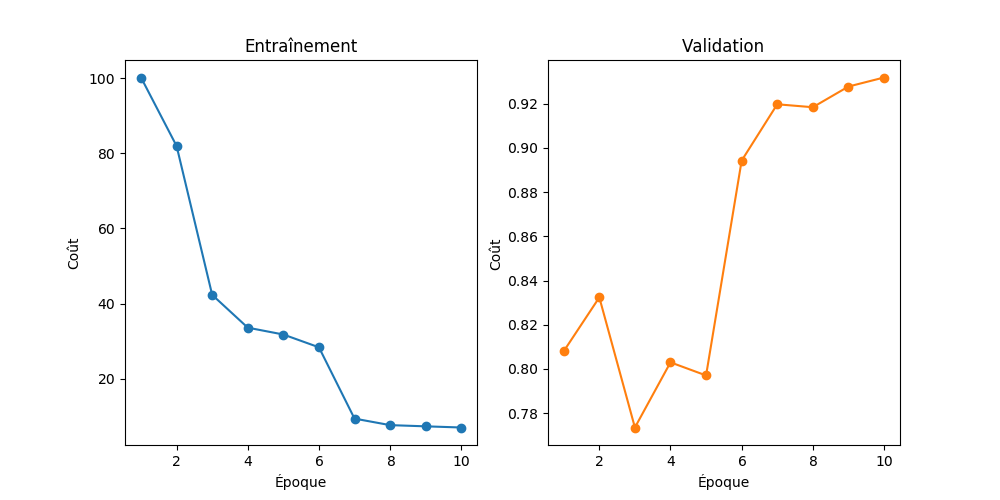
\includegraphics[width=16cm]{images/learning_curves_a.png}
        \caption{Exemple de courbe d'apprentissage du modèle A}
        \label{fig:learning_curves_a}
    \end{figure}

    \begin{figure}
        \centering
        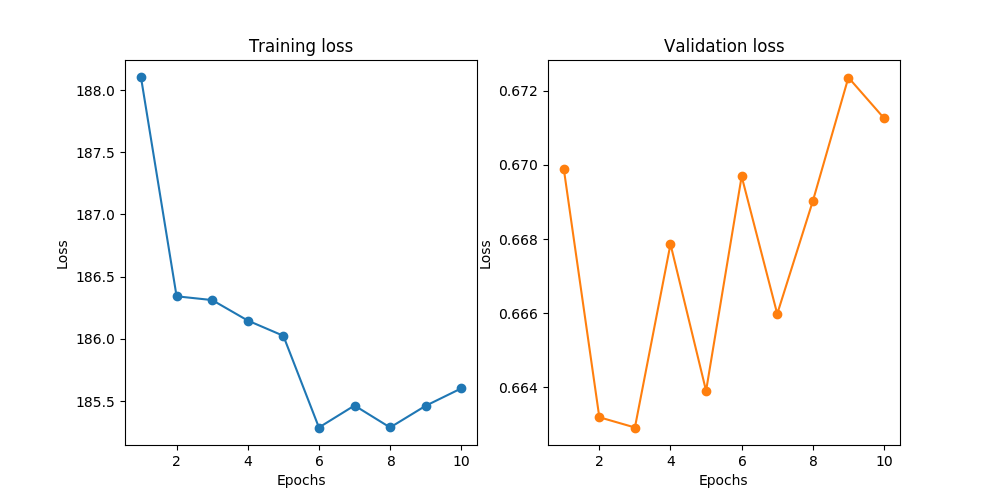
\includegraphics[width=16cm]{images/learning_curves_b.png}
        \caption{Exemple de courbe d'apprentissage du modèle B}
        \label{fig:learning_curves_b}
    \end{figure}

    \begin{figure}
        \centering
        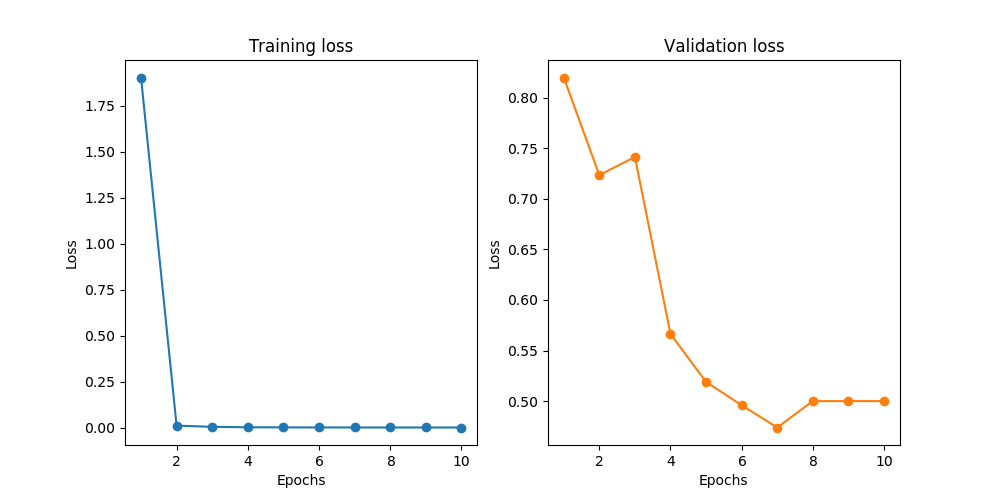
\includegraphics[width=16cm]{images/learning_curves_c.png}
        \caption{Exemple de courbe d'apprentissage du modèle C}
        \label{fig:learning_curves_c}
    \end{figure}

    \begin{figure}
        \centering
        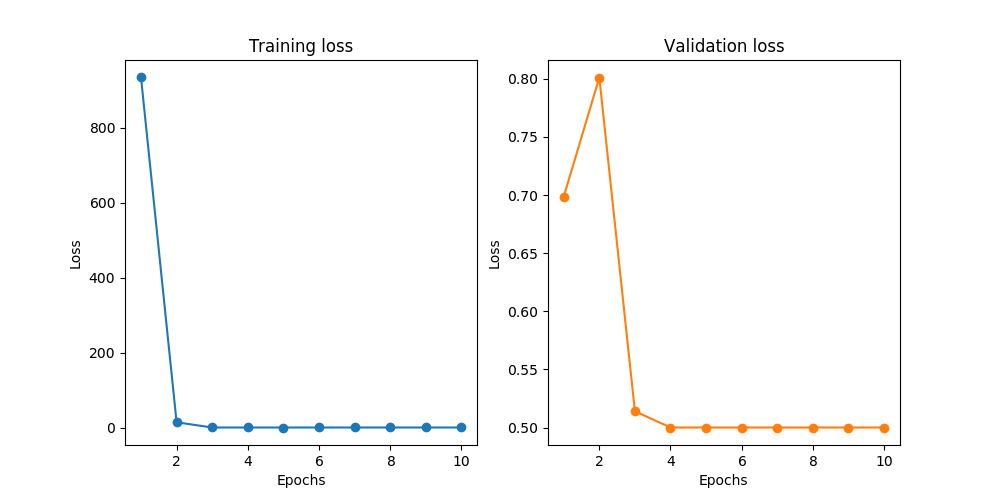
\includegraphics[width=16cm]{images/learning_curves_d.png}
        \caption{Exemple de courbe d'apprentissage du modèle D}
        \label{fig:learning_curves_d}
    \end{figure}

    \begin{figure}
        \centering
        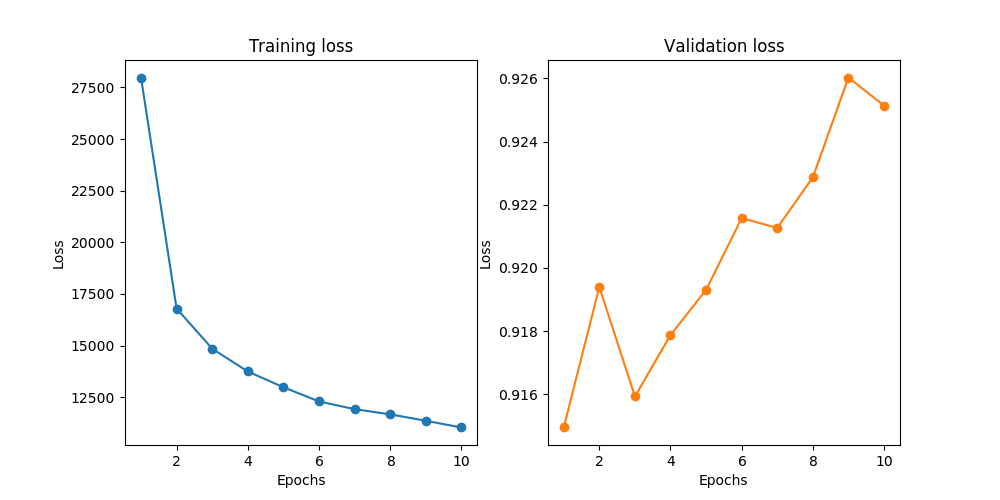
\includegraphics[width=16cm]{images/learning_curves_e.png}
        \caption{Exemple de courbe d'apprentissage du modèle E}
        \label{fig:learning_curves_e}
    \end{figure}

\subsection{Base de données - Tunnel}
    Une recherche des hyperparamètres et des tests ont été effectués pour déterminer les meilleures configurations des modèles et le meilleur modèle sur la base de données tunnel.

\subsubsection{Recherche des hyperparamètres}
    Le tableau \ref{tab:resultat_tunnel_modele_a} présente les résultats de la recherche des hyperparamètres pour le modèle A sur les images de validation de la base de données tunnel. Les configurations 5 à 10 donnent des performances sensiblement équivalentes, tandis que celles des configurations 1 à 4 sont moins bonnes. Ces dernières sont les configurations donnant un modèle avec moins de paramètres. Alors, il est possible de conclure que le modèle doit avoir assez de paramètres pour avoir de bonnes performances et que la configuration 8 est la meilleure.\\
    
    \begin{table}
        \centering
        \caption{Résultats de la recherche des hyperparamètres du modèle A - Tunnel}
        \label{tab:resultat_tunnel_modele_a}
        \begin{tabular}{lllp{3cm}p{3cm}l}
            \midrule
            \# & \(N_A\) & \(N_B\) & Augmentation des données & Métrique de validation & Époque\\
            \midrule\midrule
            1  & 2 & 2 & Non & 0,812 & 10\\
            2  & 2 & 2 & Oui & \\
            3  & 2 & 3 & Non & 0,614 & 1\\
            4  & 2 & 3 & Oui & 0,791 & 7\\
            5  & 4 & 2 & Non & 0,933 & 7\\
            6  & 4 & 2 & Oui & 0,932 & 10\\
            7  & 4 & 3 & Non & 0,930 & 7\\
            \textbf{8}  & \textbf{4} & \textbf{3} & \textbf{Oui} & \textbf{0,936} & \textbf{10}\\
            9  & 8 & 2 & Non & 0,934 & 4\\
            10 & 8 & 2 & Oui & 0,935 & 10\\
            \midrule
        \end{tabular}
    \end{table}

    Les résultats de la recherche des hyperparamètres du modèle B sont présentés dans le tableau \ref{tab:resultat_tunnel_modele_b}. L'ensemble des configurations donne des résultats semblables, mais la configuration 6 est la meilleure.\\

    \begin{table}
        \centering
        \caption{Résultats de la recherche des hyperparamètres du modèle B - Tunnel}
        \label{tab:resultat_tunnel_modele_b}
        \begin{tabular}{lllp{3cm}p{3cm}l}
            \midrule
            \# & \(N_A\) & \(N_B\) & Augmentation des données & Métrique de validation & Époque\\
            \midrule\midrule
            1  & 2 & 2 & Non & 0,612 & 9\\
            2  & 2 & 2 & Oui & 0,673 & 10\\
            3  & 2 & 3 & Non & 0,634 & 1\\
            4  & 2 & 3 & Oui & 0,673 & 6\\
            5  & 4 & 2 & Non & 0,613 & 6\\
            \textbf{6}  & \textbf{4} & \textbf{2} & \textbf{Oui} & \textbf{0,673} & \textbf{2}\\
            7  & 4 & 3 & Non & 0,621 & 4\\
            8  & 4 & 3 & Oui & 0,672 & 9\\
            9  & 8 & 2 & Non & 0,632 & 2\\
            10 & 8 & 2 & Oui & 0,672 & 6\\
            \midrule
        \end{tabular}
    \end{table}

    Le tableau \ref{tab:resultat_tunnel_modele_e} permet de constater que l'entraînement du \textit{backend} VGG16 cause une détérioration significative des performances. Ceci est possiblement relié à la détérioration des performances de validation au fil de l'entraînement des modèles C et D. Lorsqu'il y a entraînement du \textit{backend} VGG16, l'extraction des caractéristiques est détériorée, car la méthode d'entraînement ne permet pas l'apprentissage de ceci. La configuration 1 est la meilleure.\\

    \begin{table}
        \centering
        \caption{Résultats de la recherche des hyperparamètres du modèle E - Tunnel}
        \label{tab:resultat_tunnel_modele_e}
        \begin{tabular}{lp{3cm}p{3cm}p{3cm}l}
            \midrule
            \# & Entraînement du \text{backend} & Augmentation des données & Métrique de validation & Époque\\
            \midrule\midrule
            \textbf{1} & \textbf{Non} & \textbf{Non} & \textbf{0,931} & \textbf{10}\\
            2 & Non & Oui & 0,926 & 9\\
            3 & Oui & Non & 0,500 & 8\\
            4 & Oui & Oui & 0,500 & 7\\
            \midrule
        \end{tabular}
    \end{table}

\subsubsection{Comparaison entre les modèles}
    Les meilleures configurations des modèles A, B et E ont été testées sur les images de test de la base de données tunnel. Les courbes ROC présentées à la figure \ref{fig:tunnel_roc} ont été obtenues à partir de ces tests. Une autre métrique de comparaison intéressante pour comparer les différents modèles est le temps d'exécution. Le tableau \ref{tab:resultat_tunnel_temps_execution} présente les temps d'exécution moyens pour la propagation avant, la propagation arrière et total pour chacun des modèles sur une carte Tesla K20. À partir de ces informations, il est possible de conclure que le meilleur modèle pour cette base de données est le E parce que l'aire sous la courbe ROC est la plus grande et que son temps d'exécution est le moins élevé. À partir de ces résultats, il est possible d'invalider l'hypothèse énoncée par rapport à l'auto-encodeur variationnel (modèle B). Le fait de contraindre la sortie de l'encodeur détériore les performances que ce soit pour la courbe ROC ou pour le temps d'exécution.
    
    \begin{figure}
        \centering
        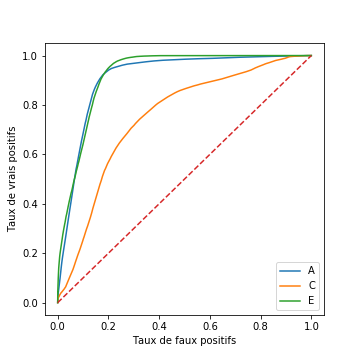
\includegraphics[width=8cm]{images/tunnel_roc.png}
        \caption{Courbes ROC - Tunnel}
        \label{fig:tunnel_roc}
    \end{figure}

    \begin{table}
        \centering
        \caption{Temps d'exécution moyens sur Tesla K20 - Tunnel}
        \label{tab:resultat_tunnel_temps_execution}
        \begin{tabular}{lp{4cm}p{4cm}p{4cm}}
            \midrule
            Modèle & Temps d'exécution moyen de la propagation avant (ms) & Temps d'exécution moyen de la propagation arrière (ms) & Temps d'exécution total moyen (ms)\\
            \midrule\midrule
            A & 2,93 & 4,75 & 7,68\\
            B & 3,65 & 5,86 & 9,51\\
            E & 3,14 & 2,78 & 5,92\\
            \midrule
        \end{tabular}
    \end{table}

\subsection{Base de données - Faculté de génie}
    Une même recherche des hyperparamètres a été effectuée sur la base de données faculté de génie pour s'assurer que les mêmes configurations des modèles permettre d'atteindre les meilleures performances. Puisque la base de données est jugée plus difficile, il est attendu que la performance des modèles soit moins bonne que celle avec la base de données tunnel.
    
\subsubsection{Recherche des hyperparamètres}
    Le tableau \ref{tab:resultat_corridor_modele_a} présente les résultats de la recherche des hyperparamètres du modèle A sur les images de validation de la base de données faculté de génie. Il est possible de constater que la configuration 5 est la meilleure. C'est une configuration différente que lors de la recherche des hyperparamètres avec la base de données tunnel. Cependant, la meilleure configuration du modèle A sur cette dernière est la configuration 8 qui a des performances semblables à la configuration 5. Comparativement aux résultats du modèle A sur la base de données tunnel, l'ensemble des configurations performent de façon semblable, sauf pour la configuration 1.\\
    
    \begin{table}
        \centering
        \caption{Résultats de la recherche des hyperparamètres du modèle A - Faculté de génie}
        \label{tab:resultat_corridor_modele_a}
        \begin{tabular}{lllp{3cm}p{3cm}l}
            \midrule
            \# & \(N_A\) & \(N_B\) & Augmentation des données & Métrique de validation & Époque\\
            \midrule\midrule
            1  & 2 & 2 & Non & 0,501 & 1\\
            2  & 2 & 2 & Oui & 0,610 & 7\\
            3  & 2 & 3 & Non & 0,665 & 8\\
            4  & 2 & 3 & Oui & 0,644 & 10\\
            \textbf{5}  & \textbf{4} & \textbf{2} & \textbf{Non} & \textbf{0,678} & \textbf{10}\\
            6  & 4 & 2 & Oui & 0,652 & 10\\
            7  & 4 & 3 & Non & 0,677 & 10\\
            8  & 4 & 3 & Oui & 0,666 & 7\\
            9  & 8 & 2 & Non & 0,667 & 9\\
            10 & 8 & 2 & Oui & 0,672 & 10\\
            \midrule
        \end{tabular}
    \end{table}
    
    Sur une base de données jugée plus difficile, les performances du modèle B présenté dans le tableau \ref{tab:resultat_corridor_modele_b} sont semblables à un modèle aléatoire (métrique de validation = 0,5) peu importe la configuration. Il n'y a que de très petites différences entre les valeurs de la métrique de validation des configurations du modèle B. Ceci est cohérent avec les résultats obtenus sur l'autre base de données. Cependant, la meilleure configuration n'est pas la même en fonction de la base de données. La configuration 5 est la meilleure sur la base de données faculté de génie, mais elle n'offre pas des performances bien meilleures qu'un modèle aléatoire.\\
    
    \begin{table}[H]
        \centering
        \caption{Résultats de la recherche des hyperparamètres du modèle B - Faculté de génie}
        \label{tab:resultat_corridor_modele_b}
        \begin{tabular}{lllp{3cm}p{3cm}l}
            \midrule
            \# & \(N_A\) & \(N_B\) & Augmentation des données & Métrique de validation & Époque\\
            \midrule\midrule
            1  & 2 & 2 & Non & 0,499 & 7\\
            2  & 2 & 2 & Oui & 0,503 & 5\\
            3  & 2 & 3 & Non & 0,499 & 10\\
            4  & 2 & 3 & Oui & 0,502 & 4\\
            \textbf{5}  & \textbf{4} & \textbf{2} & \textbf{Non} & \textbf{0,511} & \textbf{1}\\
            6  & 4 & 2 & Oui & 0,501 & 10\\
            7  & 4 & 3 & Non & 0,501 & 8\\
            8  & 4 & 3 & Oui & 0,500 & 2\\
            9  & 8 & 2 & Non & 0,499 & 1\\
            10 & 8 & 2 & Oui & 0,501 & 10\\
            \midrule
        \end{tabular}
    \end{table}
    
    Le tableau \ref{tab:resultat_corridor_modele_e} présente les résultats de la recherche des hyperparamètres du modèle E sur la base de données faculté de génie. La même configuration que celle sur l'autre base de données offre les meilleures performances pour le modèle E.\\
    
    \begin{table}[H]
        \centering
        \caption{Résultats de la recherche des hyperparamètres du modèle E - Faculté de génie}
        \label{tab:resultat_corridor_modele_e}
        \begin{tabular}{lp{3cm}p{3cm}p{3cm}l}
            \midrule
            \# & Entraînement du \text{backend} & Augmentation des données & Métrique de validation & Époque\\
            \midrule\midrule
            \textbf{1} & \textbf{Non} & \textbf{Non} & \textbf{0,719} & \textbf{10}\\
            2 & Non & Oui & 0,699 & 7\\
            3 & Oui & Non & 0,500 & 10\\
            4 & Oui & Oui & 0,500 & 10\\
            \midrule
        \end{tabular}
    \end{table}

\subsubsection{Comparaison entre les modèles}
    Comme avec l'autre base de données, les courbes ROC et les temps d'exécution ont été calculés pour la meilleure configuration de chacun des modèles sur les images de tests de la base de données faculté de génie. Ces informations sont présentées dans la figure \ref{fig:corridor_roc} et le tableau \ref{tab:resultat_corridor_temps_execution}. Le meilleur modèle pour cette base de données est le même que pour l'autre. Le modèle E est le meilleur parce qu'il a le temps d'exécution le plus petit et l'aire sous la courbe ROC à la plus grande. De façon générale, les trois modèles ont moins bien performé sur cette base de données que sur l'autre parce que leur aire sous la courbe est bien moins grande. Les résultats du modèle B sur la base de données faculté de génie enforcit l'invalidation énoncée par rapport à l'auto-encodeur variationnel (modèle B).
    
    \begin{figure}[H]
        \centering
        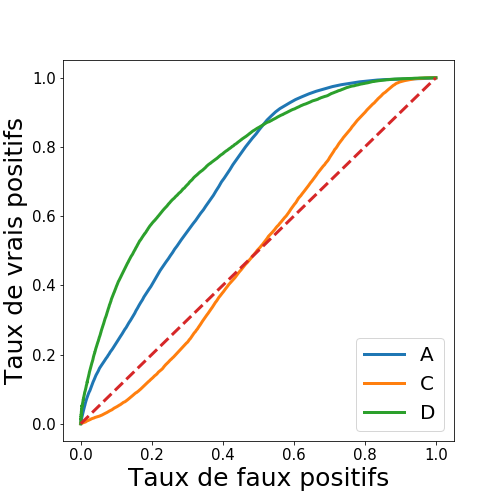
\includegraphics[width=8cm]{images/corridor_roc.png}
        \caption{Courbes ROC - Faculté de génie}
        \label{fig:corridor_roc}
    \end{figure}

    \begin{table}[H]
        \centering
        \caption{Temps d'exécution moyens sur Tesla K20 - Faculté de génie}
        \label{tab:resultat_corridor_temps_execution}
        \begin{tabular}{lp{4cm}p{4cm}p{4cm}}
            \midrule
            Modèle & Temps d'exécution moyen de la propagation avant (ms) & Temps d'exécution moyen de la propagation arrière (ms) & Temps d'exécution total moyen (ms)\\
            \midrule\midrule
            A & 3,08 & 4,22 & 7,30\\
            B & 3,65 & 5,86 & 9,51\\
            E & 3,14 & 2,78 & 5,92\\
            \midrule
        \end{tabular}
    \end{table}
    
\subsection{Visualisation des régions sur les images de tests}
    Afin de rendre les résultats facilement interprétables, des séquences vidéos ont été générées à partir des images annotées par le modèle E. Les images annotées manuellement et ayant servi à établir les métriques de performances ont été juxtaposées aux images annotées par le modèle.\\

    Les figures \ref{fig:frame_corridor} et \ref{fig:frame_tunnel} donnent un aperçu des performances sur les images de tests des bases de données tunnel et faculté de génie respectivement. Le modèle peut être utilisé avec un seuil d'excitation paramétrable. Ce seuil est comparé avec l'erreur de reconstruction sortant des modèles. Il a été nécessaire d'établir le seuil à partir duquel le modèle devient \textit{curieux}, et à partir duquel sont déterminées les régions d’intérêt annotées en rouge sur l'image. En l’occurrence, le seuil a été ajusté à une valeur de 2,5 déterminé empiriquement à l'aide des courbes ROC. Une valeur arbitraire permettant d'atteindre un ratio de 90\% de vrais positifs pour 16\% de faux positifs sur les images de tests de la base de données tunnel, et de 62\% de vrais positifs pour 23\% de faux positifs sur la base de données faculté de génie. Ces vidéos sont jointes dans l'archive contenant le présent rapport.\\

    \begin{figure}
        \centering
        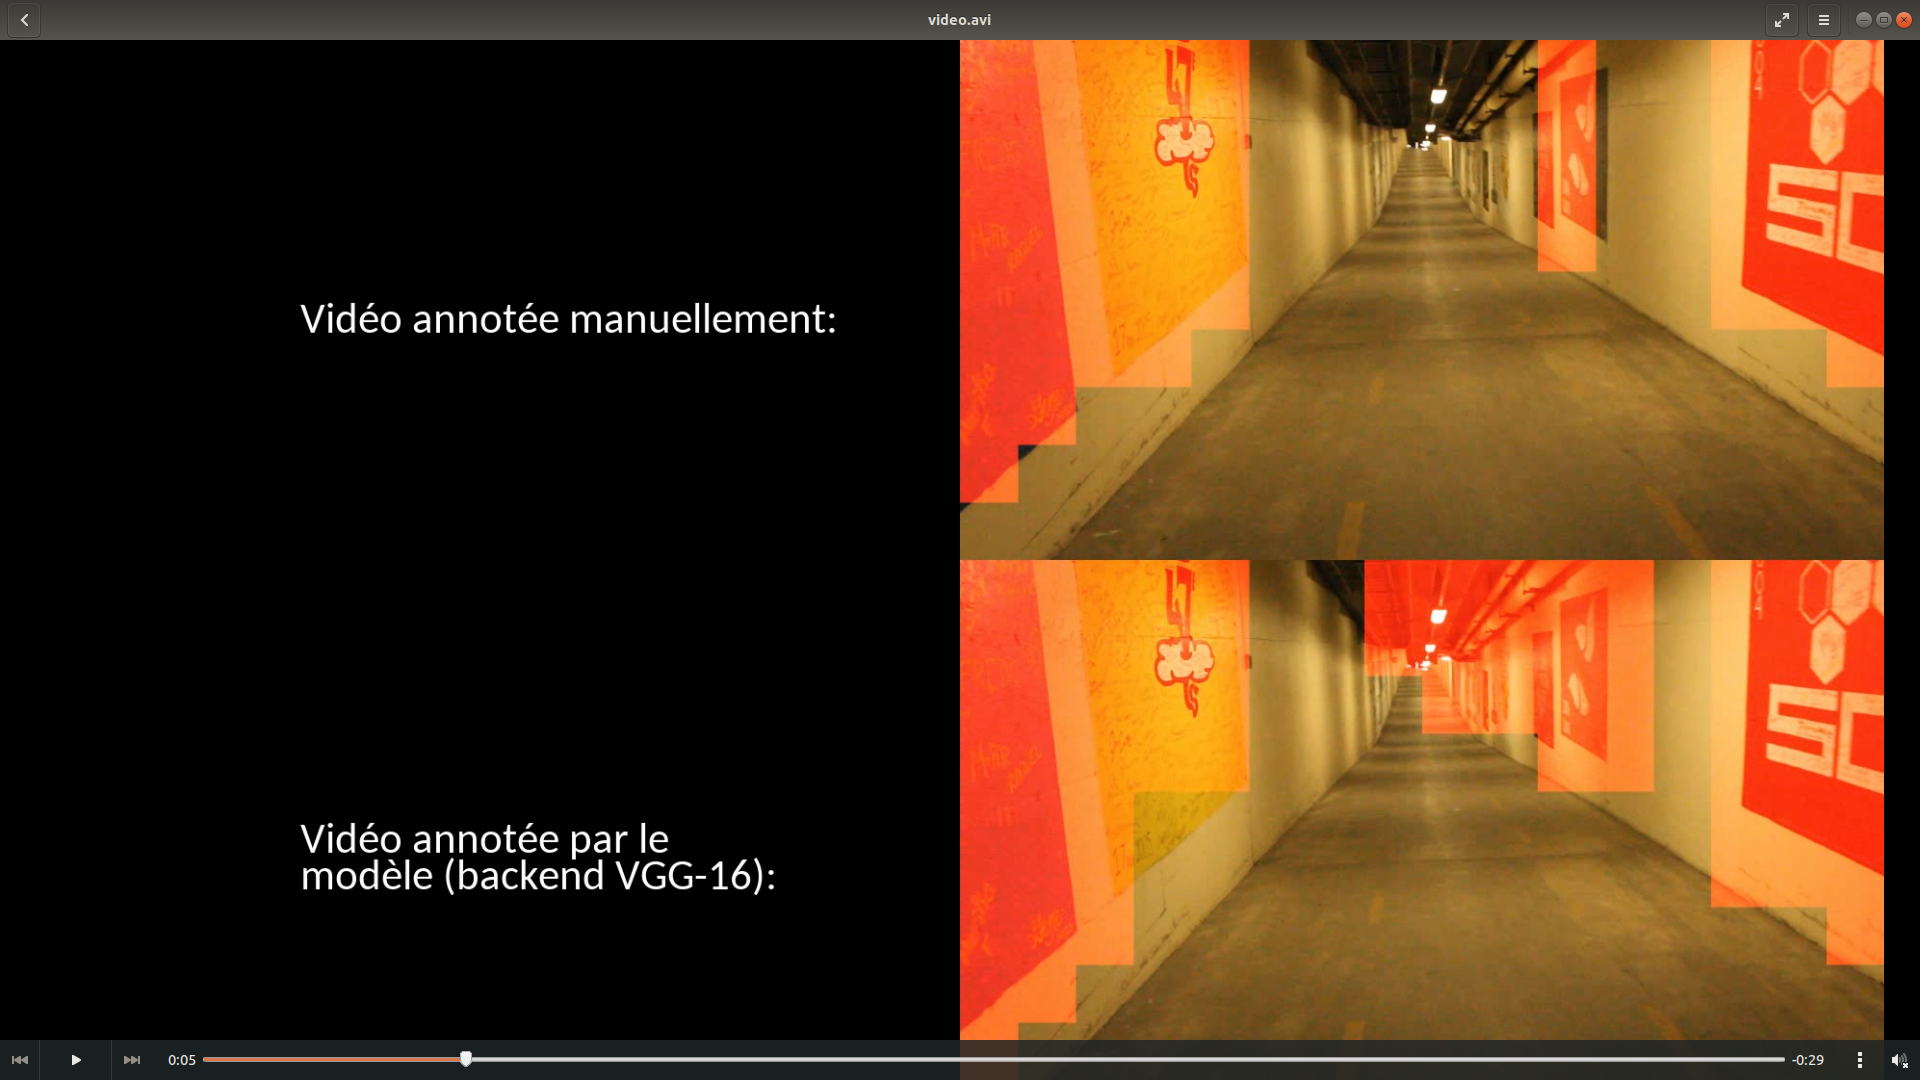
\includegraphics[width=17cm]{images/frame_tunnel.png}
        \caption{Capture d'écran de la vidéo générée par le modèle entraîné et testé avec les images de la base de données tunnel}
        \label{fig:frame_tunnel}
    \end{figure}

    La figure \ref{fig:frame_tunnel} montre la performance du modèle entraîné et testé avec les images de la base de données tunnel. Le modèle est en mesure de discerner la présence de fresques sur les murs du tunnel. Par ailleurs, on constate qu'il méprend la tuyauterie et les lumières au plafond avec des affiches. Le modèle interprète parfois l'extrémité du tunnel devant lui comme un élément d'intérêt, alors qu'il est également présent dans les images d'entraînement. Dans certaines images, on peut également voir que le modèle s’intéresse à des éléments se trouvant sur le sol, alors que ceux-ci étaient également présents dans les images d'entraînement.\\

    \begin{figure}
        \centering
        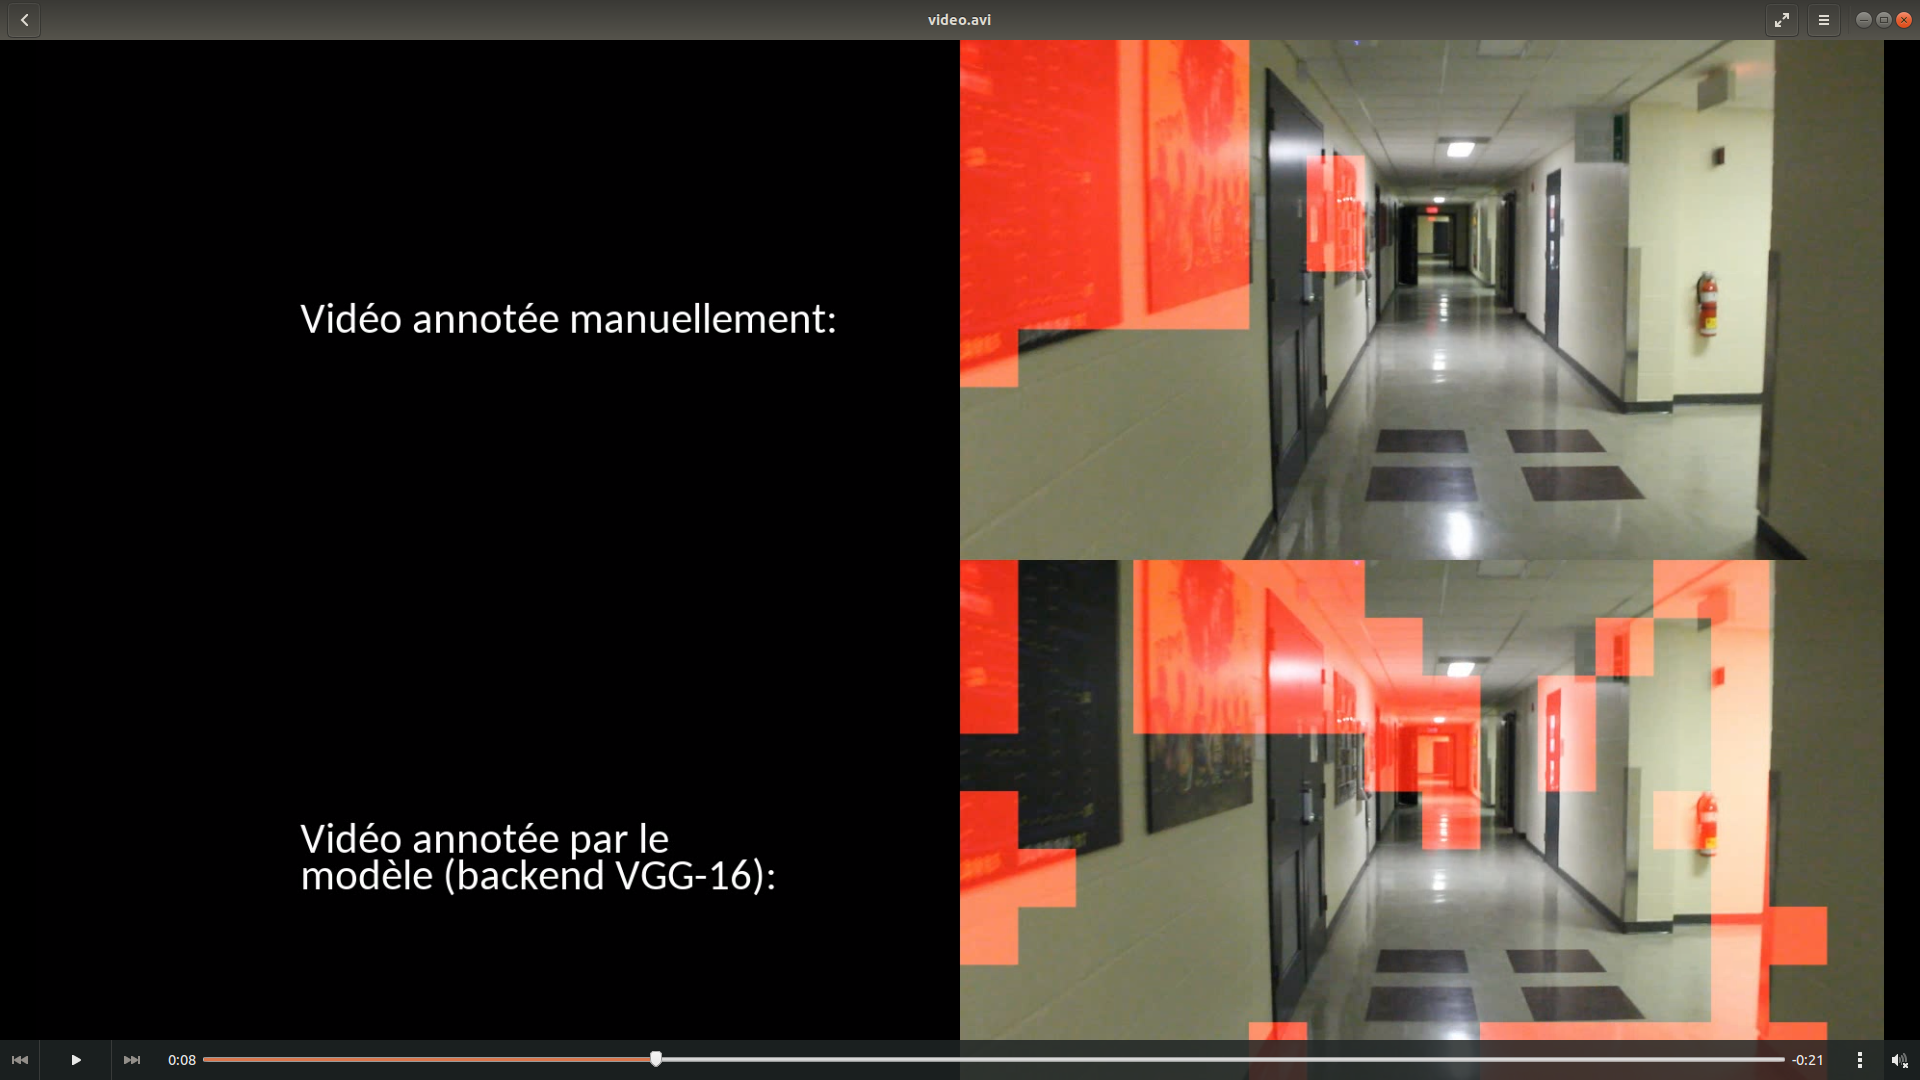
\includegraphics[width=17cm]{images/frame_corridor.png}
        \caption{Capture d'écran de la vidéo générée par le modèle entraîné et testé avec les images de la base de données faculté de génie}
        \label{fig:frame_corridor}
    \end{figure}

    La figure \ref{fig:frame_corridor} permet de constater que dans la base de données faculté de génie, le modèle peine à discriminer les éléments hétéroclites qu'il perçoit dans son environnement. La grande diversité d'éléments le confond. En effet, ceux-ci n'ont pas fait l'objet d'annotations manuelles, mais présentent néanmoins certains attributs communs avec les panneaux. L'auto-encodeur a généré un signal d’intérêt en se fiant à des environnements moins diversifiés. En rétrospective, l'annotation manuelle ayant servi à établir un comparatif aurait probablement pu être améliorée en prenant en compte davantage d'éléments pouvant susciter l’intérêt du modèle.\\

    Les figues \ref{fig:frame_tr_corridor_test_tunnel} et \ref{fig:frame_tr_tunnel_test_corridor} montrent les résultats des annotations produites par le modèle lorsque entraîné avec les images de la base de données faculté de génie et testé sur l'autre base de données, et lorsque entraîné avec les images de la base de données tunnel et testé sur l'autre base de données. Dans les deux cas, on peut constater une baisse de la performance par rapport aux entraînements et tests effectués avec les mêmes images. Ceci suggère une faible capacité de généralisation du modèle entre différents environnements similaires, et donc un seuil trop bas pour la génération du signal de curiosité. Autrement dit, l'erreur de reconstruction de l'auto-encodeur est augmentée lorsqu'on passe d'un environnement à l'autre.\\

    \begin{figure}
        \centering
        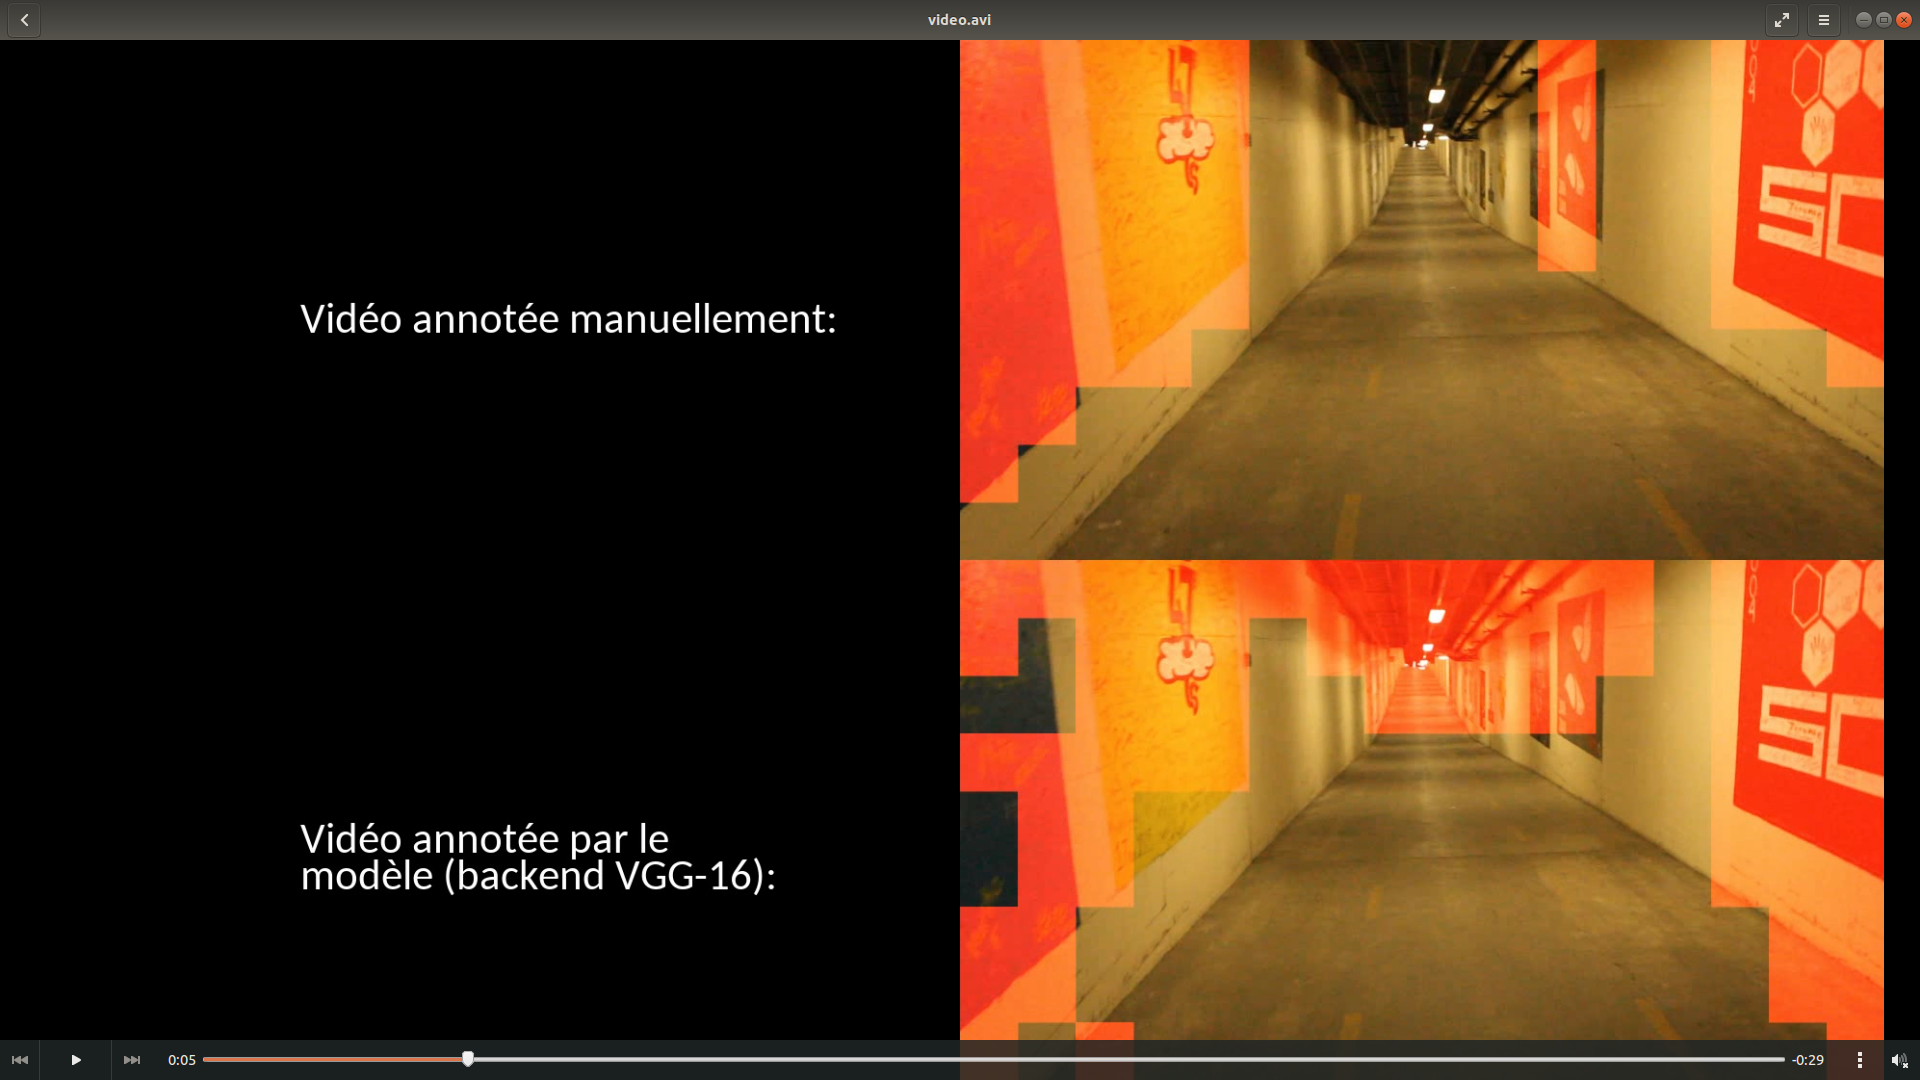
\includegraphics[width=17cm]{images/frame_tr_corridor_test_tunnel.png}
        \caption{Capture d'écran de la vidéo générée par le modèle entraîné avec les images de la base de données faculté de génie et testé avec les images de la base de données tunnel}
        \label{fig:frame_tr_corridor_test_tunnel}
    \end{figure}

    \begin{figure}
        \centering
        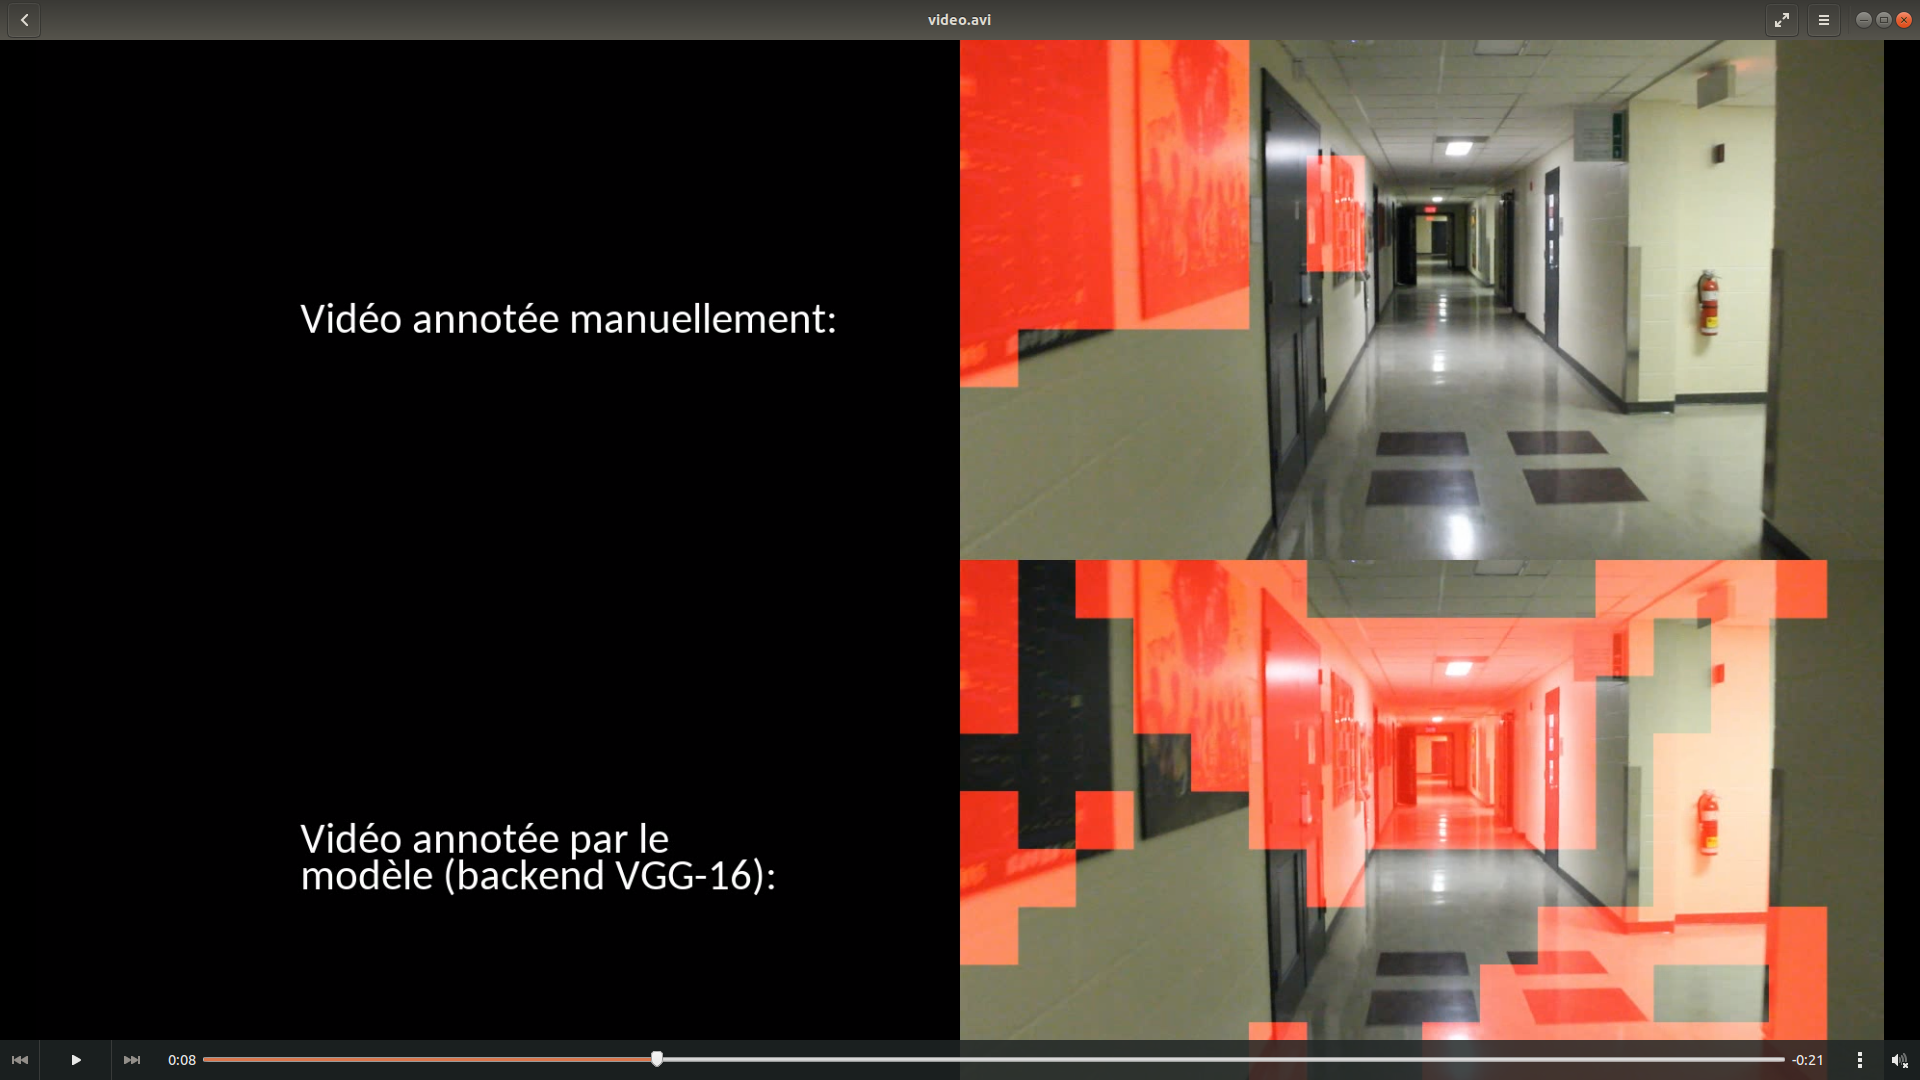
\includegraphics[width=17cm]{images/frame_tr_tunnel_test_corridor.png}
        \caption{Capture d'écran de la vidéo générée par le modèle entraîné avec les images de la base de données tunnel et testé avec les images de la base de données faculté de génie}
        \label{fig:frame_tr_tunnel_test_corridor}
    \end{figure}
    
\subsection{Analyse générale}
    Lors de la recherche des hyperparamètres, toutes les configurations des modèles ont été testées avec et sans l'augmentation des données dans le but de déterminer si c'était bénéfique d'utiliser cette technique dans ce contexte. À partir de tous les tableaux présentant les résultats de la recherche des hyperparamètres, il n'est pas possible d'affirmer que l'augmentation des données est bénéfique ou non, car pour certains cas cette technique améliore un peu les performances de validation et pour d'autres il y a une détérioration.\\
    
    Tous les résultats obtenus à partir des images de test permettent de conclure que l'erreur de reconstruction d'un auto-encodeur travaillant sur les pixels ou les caractéristiques peut être utilisée comme signal de curiosité pour un mécanisme d'attention d'un robot. Cependant, la complexité de l'environnement dans lequel le robot interagit ne doit pas trop être complexe, sinon le taux de faux positifs devient bien trop important. Même si l'environnement n'est pas complexe, le taux de faux positifs n'est pas de zéro, donc le système d'attention ne doit pas être sensible aux faux positifs. Le modèle E est conseillé, car il offre les meilleures performances et le plus faible temps d'exécution sur les deux bases de données.